% Supplied prototype measurements; green denotes additions to the report.
\subsection{Preliminary Prototype Current and LoRa Power Measurements}
\label{sec:measured_power}
\newrevision{The preliminary power tests recorded current in several prototype operating modes and measured LoRa transmission current at four transmit-power settings with a 3.3 V supply. Battery life still requires measured sleep current, activity durations, converter losses, and a complete duty-cycle test.}

\begin{table}[htbp]
\centering
\caption{\newrevision{Corrected prototype operating currents recorded on 7 November 2026.}}
\label{tab:mode_current}
\begin{tabular}{lrrrr}
\toprule
Mode & Total (mA) & Increment (mA) & Time (s) & Supply (V) \\
\midrule
Idle & 33 & 0 & 60 & 4.8 \\
Sensing & 42 & 9 & 60 & 4.8 \\
CNN active & 53 & 20 & 60 & --- \\
CNN idle & 33 & 0 & 60 & --- \\
Radio standby & 33 & 0 & --- & --- \\
Deep sleep & --- & --- & --- & 5.0 input \\
\bottomrule
\end{tabular}
\end{table}

\newrevision{All non-transmission readings include the ESP32 and the connected circuitry or active workload. The incremental estimate is $\Delta I=I_{\mathrm{mode}}-33$ mA, using idle current as a common baseline. This estimates additional system current rather than isolated component consumption. CNN active is 20 mA above CNN idle. Dashes indicate unrecorded values.}

\newrevision{The updated operating-current readings were obtained using a different multimeter. Supply voltage remains unrecorded for CNN and standby modes. These are readings at the time observed, not averages over the listed durations. At 4.8 V, idle and sensing power are 158.4 and 201.6 mW, with a 43.2 mW increment. Equal indicated currents do not establish zero component consumption. Measurement accuracy has not been quantified.}

\newrevision{The CNN-active measurement used repeated inference on a fixed test input with the \texttt{stream1s\_w8\_d4} model. The radio standby measurement used the SX1278 standby mode. Both readings characterize individual operating states.}

\newrevision{Deep-sleep current and power have not been measured for the assembled system. At the nominal 5 V board input, a measured sleep current $I_{\mathrm{sleep}}$ in mA gives $P_{\mathrm{sleep}}=5I_{\mathrm{sleep}}$ mW. This must include the board, regulator, sensor, and radio in their actual sleep states; no numeric sleep value is assigned.}

\begin{figure}[htbp]
\centering
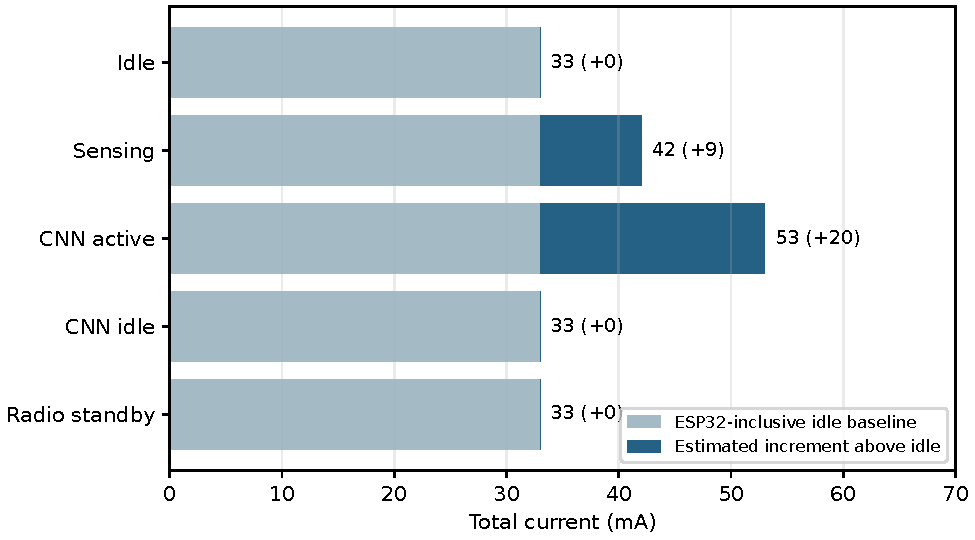
\includegraphics[width=0.9\textwidth]{figures/operating_mode_current.pdf}
\caption{\newrevision{ESP32-inclusive readings split into the 33 mA idle baseline and estimated increments. Equal indicated readings do not establish zero component consumption.}}
\label{fig:mode_current}
\end{figure}

\begin{table}[htbp]
\centering
\caption{\newrevision{LoRa transmission current at 3.3 V and calculated power and energy. Energy calculations use the full indicated current.}}
\label{tab:lora_power}
\begin{tabular}{rrrrrr}
\toprule
TX setting & Current & Power & Run energy & Packet energy & DATA energy \\
(dBm) & (mA) & (mW) & (J) & (mJ) & (mJ/byte) \\
\midrule
10 & 20 & 66 & 2.8 & 2.8 & 0.35 \\
15 & 30 & 99 & 4.2 & 4.2 & 0.52 \\
17 & 40 & 132 & 5.5 & 5.5 & 0.69 \\
19 & 60 & 198 & 8.3 & 8.3 & 1.04 \\
\bottomrule
\end{tabular}
\end{table}

\newrevision{Measurement repeatability and instrument accuracy remain unquantified. The table reports rounded energy values.}

\newrevision{Power is calculated as $P=VI$, run energy as $E=Pt$, and energy per packet as $E/N$, using a 42 s run and 1,000 transmitted packets per setting. Energy per DATA byte divides packet energy by eight, the DATA packet length in this experiment. The calculations assume the indicated current represents the run average. The measurement instrument, repetition count, radio parameters, receiver delivery count, and measurement boundary remain undocumented. The results estimate run energy and energy per transmitted packet and DATA byte.}

\begin{figure}[htbp]
\centering
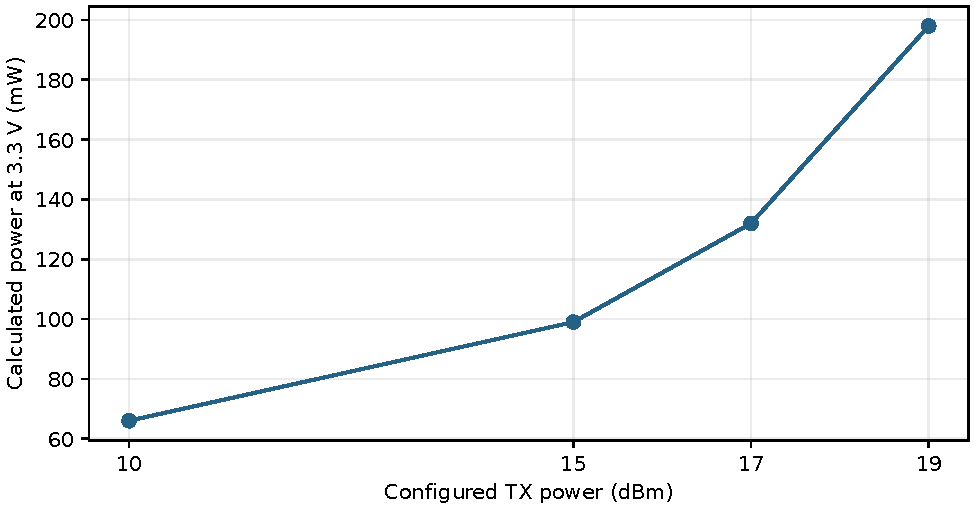
\includegraphics[width=0.9\textwidth]{figures/lora_power_sweep.pdf}
\caption{\newrevision{Calculated LoRa power at a 3.3 V supply for four transmit-power settings.}}
\label{fig:lora_power_sweep}
\end{figure}

\newrevision{Calculated power rises from 66 mW at 10 dBm to 198 mW at 19 dBm, a threefold increase. Selecting a TX setting also requires packet-delivery and range measurements under the permitted local radio settings. The 3.3 V sweep and the operating-mode measurements characterize separate test setups. Comparing their readings requires equivalent supply conditions and measurement boundaries.}
\FloatBarrier
